\documentclass{tufte-book}

%%
% Book metadata
\title{A Tufte-Style Book\thanks{Thanks to Edward R.~Tufte for his inspiration.}}
\author[The Tufte-LaTeX Developers]{The Tufte-LaTeX\ Developers}
\publisher{Publisher of This Book}

%%
% If they're installed, use Bergamo and Chantilly from www.fontsite.com.
% They're clones of Bembo and Gill Sans, respectively.
%\IfFileExists{bergamo.sty}{\usepackage[osf]{bergamo}}{}% Bembo
%\IfFileExists{chantill.sty}{\usepackage{chantill}}{}% Gill Sans

%\usepackage{microtype}

%%
% Just some sample text
\usepackage{lipsum}

%%
% For nicely typeset tabular material
\usepackage{booktabs}

%%
% For graphics / images
\usepackage{graphicx}

%%
% Prints argument within hanging parentheses (i.e., parentheses that take
% up no horizontal space).  Useful in tabular environments.
\newcommand{\hangp}[1]{\makebox[0pt][r]{(}#1\makebox[0pt][l]{)}}

%%
% Prints an asterisk that takes up no horizontal space.
% Useful in tabular environments.
\newcommand{\hangstar}{\makebox[0pt][l]{*}}

%%
% Prints a trailing space in a smart way.
\usepackage{xspace}

%%
% Some shortcuts for Tufte's book titles.  The lowercase commands will
% produce the initials of the book title in italics.  The all-caps commands
% will print out the full title of the book in italics.
\newcommand{\vdqi}{\textit{VDQI}\xspace}
\newcommand{\ei}{\textit{EI}\xspace}
\newcommand{\ve}{\textit{VE}\xspace}
\newcommand{\be}{\textit{BE}\xspace}
\newcommand{\VDQI}{\textit{The Visual Display of Quantitative Information}\xspace}
\newcommand{\EI}{\textit{Envisioning Information}\xspace}
\newcommand{\VE}{\textit{Visual Explanations}\xspace}
\newcommand{\BE}{\textit{Beautiful Evidence}\xspace}

\newcommand{\TL}{Tufte-\LaTeX\xspace}

% Prints the month name (e.g., January) and the year (e.g., 2008)
\newcommand{\monthyear}{%
  \ifcase\month\or January\or February\or March\or April\or May\or June\or
  July\or August\or September\or October\or November\or
  December\fi\space\number\year
}


% Prints an epigraph and speaker in sans serif, all-caps type.
\newcommand{\openepigraph}[2]{%
  %\sffamily\fontsize{14}{16}\selectfont
  \begin{fullwidth}
  \sffamily\large
  \begin{doublespace}
  \noindent\allcaps{#1}\\% epigraph
  \noindent\allcaps{#2}% author
  \end{doublespace}
  \end{fullwidth}
}

% Inserts a blank page
\newcommand{\blankpage}{\newpage\hbox{}\thispagestyle{empty}\newpage}

\usepackage{units}

% Typesets the font size, leading, and measure in the form of 10/12x26 pc.
\newcommand{\measure}[3]{#1/#2$\times$\unit[#3]{pc}}

\begin{document}

% Front matter
\frontmatter

% r.1 blank page
\blankpage

% v.2 epigraphs
\newpage\thispagestyle{empty}
\openepigraph{%
The public is more familiar with bad design than good design.
It is, in effect, conditioned to prefer bad design, 
because that is what it lives with. 
The new becomes threatening, the old reassuring.
}{Paul Rand%, {\itshape Design, Form, and Chaos}
}
\vfill
\openepigraph{%
A designer knows that he has achieved perfection 
not when there is nothing left to add, 
but when there is nothing left to take away.
}{Antoine de St-Expurey}
\vfill
\openepigraph{%
\ldots the designer of a new system must not only be the implementor and the first 
large-scale user; the designer should also write the first user manual\ldots 
If I had not participated fully in all these activities, 
literally hundreds of improvements would never have been made, 
because I would never have thought of them or perceived 
why they were important.
}{Donald E. Knuth}


% r.3 full title page
\maketitle


% v.4 copyright page
\newpage
\begin{fullwidth}
~\vfill
\thispagestyle{empty}
\setlength{\parindent}{0pt}
\setlength{\parskip}{\baselineskip}
Copyright \copyright\ \the\year\ \thanklessauthor

\par\smallcaps{Published by \thanklesspublisher}

\par\smallcaps{tufte-latex.googlecode.com}

\par Licensed under the Apache License, Version 2.0 (the ``License''); you may not
use this file except in compliance with the License. You may obtain a copy
of the License at \url{http://www.apache.org/licenses/LICENSE-2.0}. Unless
required by applicable law or agreed to in writing, software distributed
under the License is distributed on an \smallcaps{``AS IS'' BASIS, WITHOUT
WARRANTIES OR CONDITIONS OF ANY KIND}, either express or implied. See the
License for the specific language governing permissions and limitations
under the License.

\par\textit{First printing, \monthyear}
\end{fullwidth}

% r.5 contents
\tableofcontents

% r.7 dedication
\cleardoublepage
~\vfill
\begin{doublespace}
\noindent\fontsize{18}{22}\selectfont\itshape
\nohyphenation
Dedicated to those who appreciate \LaTeX{} 
and the work of \mbox{Edward R.~Tufte} 
and \mbox{Donald E.~Knuth}.
\end{doublespace}
\vfill
\vfill


% r.9 introduction
\cleardoublepage
\chapter*{Introduction}

This sample book discusses the design of Edward Tufte's
books\cite{Tufte2001,Tufte1990,Tufte1997,Tufte2006}
and the use of the \texttt{tufte-book} and \texttt{sample-handout} document classes.


%%
% Start the main matter (normal chapters)
\mainmatter


\chapter{The Design of Tufte's Books}
\label{ch:tufte-design}


\newthought{The pages} of a book are usually divided into three major
sections: the front matter (also called preliminary matter or prelim), the
main matter (the core text of the book), and the back matter (or end
matter).

\newthought{The front matter} of a book refers to all of the material that
comes before the main text.  The following table from shows a list of
material that appears in the front matter of \VDQI, \EI, \VE, and \BE
along with its page number.  Page numbers that appear in parentheses refer
to folios that do not have a printed page number (but they are still
counted in the page number sequence).

\bigskip
\begin{minipage}{\textwidth}
\begin{center}
\begin{tabular}{lcccc}
\toprule
 & \multicolumn{4}{c}{Books} \\
\cmidrule(l){2-5} 
Page content & \vdqi & \ei & \ve & \be \\
\midrule
Blank half title page & \hangp{1} & \hangp{1} & \hangp{1} & \hangp{1} \\
Frontispiece\footnotemark{}
  & \hangp{2} & \hangp{2} & \hangp{2} & \hangp{2} \\
Full title page & \hangp{3} & \hangp{3} & \hangp{3} & \hangp{3} \\
Copyright page & \hangp{4} & \hangp{4} & \hangp{4} & \hangp{4} \\
Contents & \hangp{5} & \hangp{5} & \hangp{5} & \hangp{5} \\
%Blank & -- & \hangp{6} & \hangp{6} & \hangp{6} \\
Dedication & \hangp{6} & \hangp{7} & \hangp{7} & 7 \\
%Blank & -- & \hangp{8} & -- & \hangp{8} \\
Epigraph & -- & -- & \hangp{8} & -- \\
Introduction & \hangp{7} & \hangp{9} & \hangp{9} & 9 \\
\bottomrule
\end{tabular}
\end{center}
\end{minipage}
\vspace{-7\baselineskip}\footnotetext{The contents of this page vary from book to book.  In
  \vdqi this page is blank; in \ei and \ve this page holds a frontispiece;
  and in \be this page contains three epigraphs.}
\vspace{7\baselineskip}

\bigskip
The design of the front matter in Tufte's books varies slightly from the
traditional design of front matter.  First, the pages in front matter are
traditionally numbered with lowercase roman numerals (e.g., i, ii, iii,
iv,~\ldots).  Second, the front matter page numbering sequence is usually
separate from the main matter page numbering.  That is, the page numbers
restart at 1 when the main matter begins.  In contrast, Tufte has
enumerated his pages with arabic numerals that share the same page counting
sequence as the main matter.  

There are also some variations in design across Tufte's four books.  The
page opposite the full title page (labeled ``frontispiece'' in the above
table) has different content in each of the books.  In \VDQI, this page is
blank; in \EI and \VE, this page holds a frontispiece; and in \BE, this
page contains three epigraphs.

The dedication appears on page~6 in \vdqi (opposite the introduction), and
is placed on its own spread in the other books.  In \ve, an epigraph shares
the spread with the opening page of the introduction.

None of the page numbers (folios) of the front matter are expressed except in
\be, where the folios start to appear on the dedication page.

\newthought{The full title page} of each of the books varies slightly in
design.  In all the books, the author's name appears at the top of the
page, the title it set just above the center line, and the publisher is
printed along the bottom margin.  Some of the differences are outlined in
the following table.

\bigskip
\begin{center}
\footnotesize
\begin{tabular}{lllll}
\toprule
Feature & \vdqi & \ei & \ve & \be \\
\midrule
Author & & & & \\
\quad Typeface & serif   & serif   & serif   & sans serif \\
\quad Style    & italics & italics & italics & upright, caps \\
\quad Size     & 24 pt   & 20 pt   & 20 pt   & 20 pt \\
\addlinespace
Title & & & & \\
\quad Typeface & serif   & serif   & serif   & sans serif \\
\quad Style    & upright & italics & upright & upright, caps \\
\quad Size     & 36 pt   & 48 pt   & 48 pt   & 36 pt \\
\addlinespace
Subtitle & & & & \\
\quad Typeface & --      & --      & serif   & -- \\
\quad Style    & --      & --      & upright & -- \\
\quad Size     & --      & --      & 20 pt   & -- \\
\addlinespace
Edition & & & & \\
\quad Typeface & sans serif           & --      & --      & -- \\
\quad Style    & upright, caps & --      & --      & -- \\
\quad Size     & 14 pt                & --      & --      & -- \\
\addlinespace
Publisher & & & & \\
\quad Typeface & serif   & serif   & serif   & sans serif \\
\quad Style    & italics & italics & italics & upright, caps \\
\quad Size     & 14 pt   & 14 pt   & 14 pt   & 14 pt \\
\bottomrule
\end{tabular}
\end{center}

\begin{figure*}[p]
\fbox{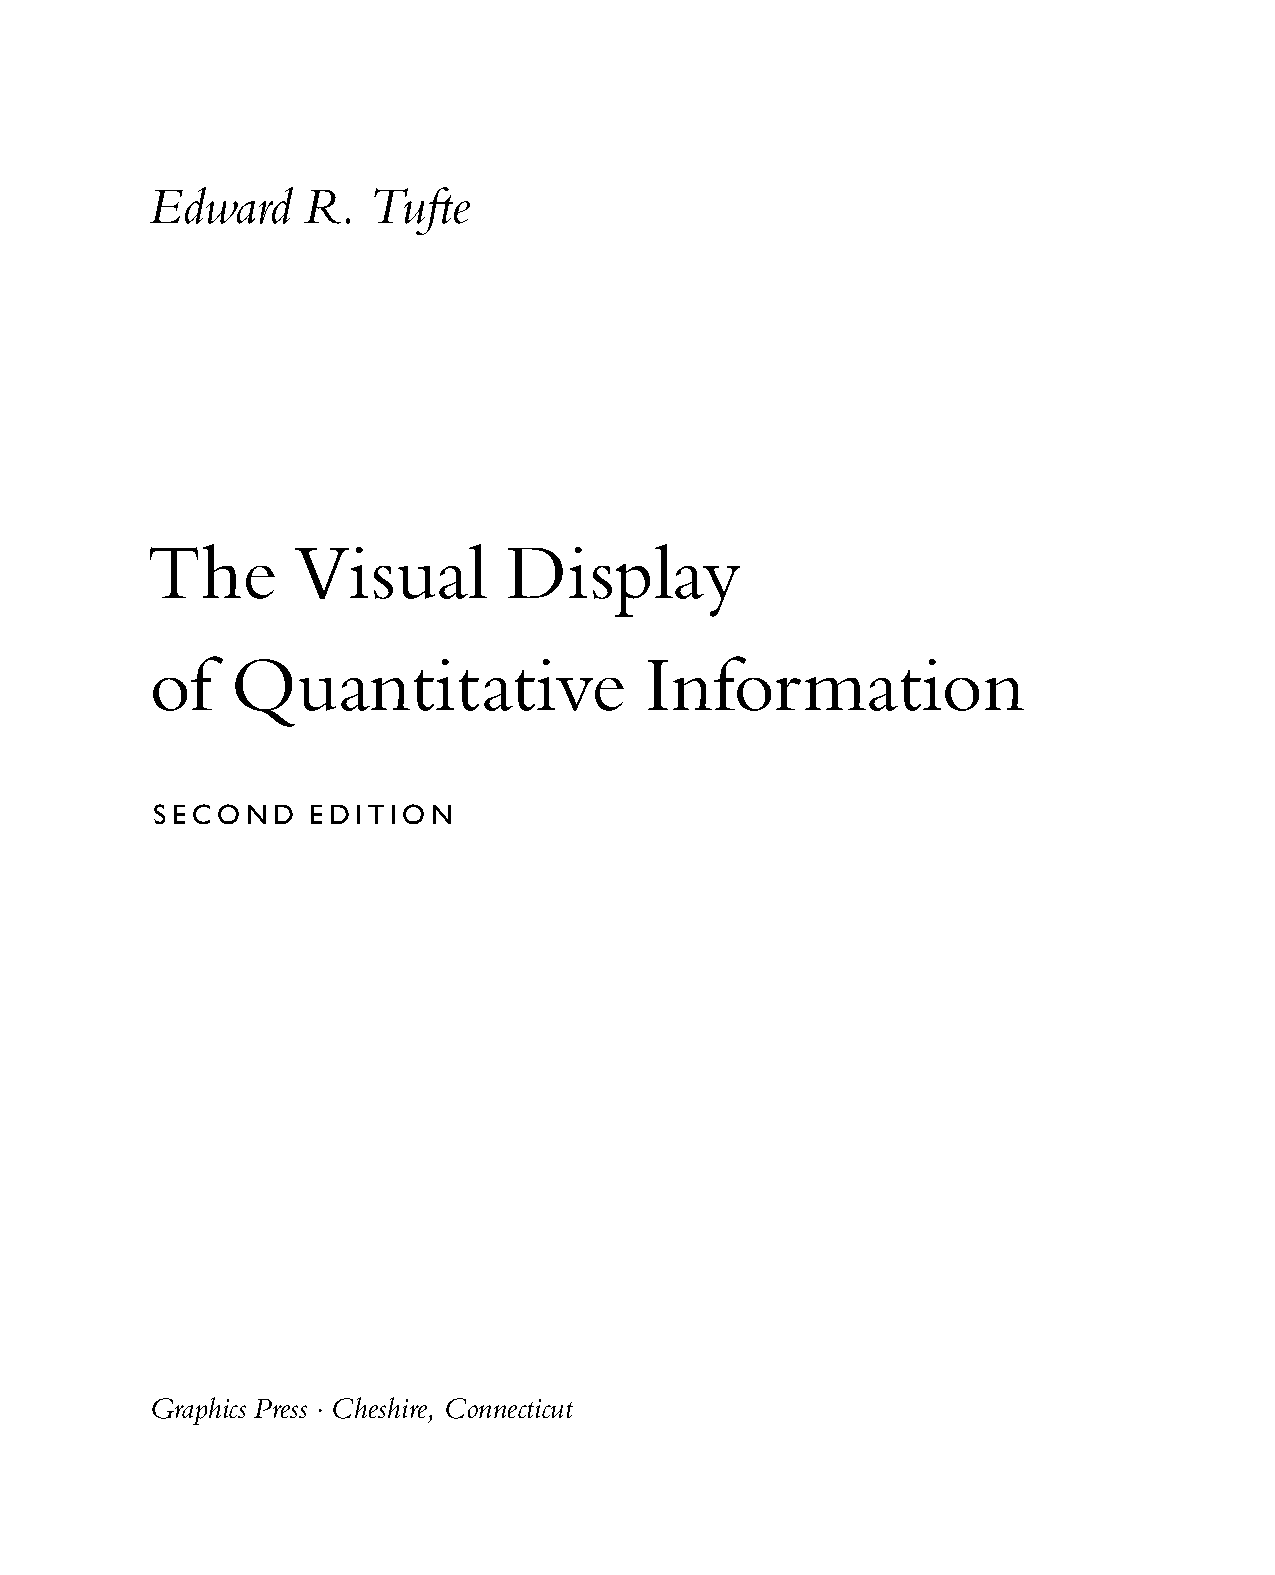
\includegraphics[width=0.45\linewidth]{graphics/vdqi-title.pdf}}
\hfill
\fbox{
\includegraphics[width=0.45\linewidth]{graphics/ei-title.pdf}}
\\\vspace{\baselineskip}
\fbox{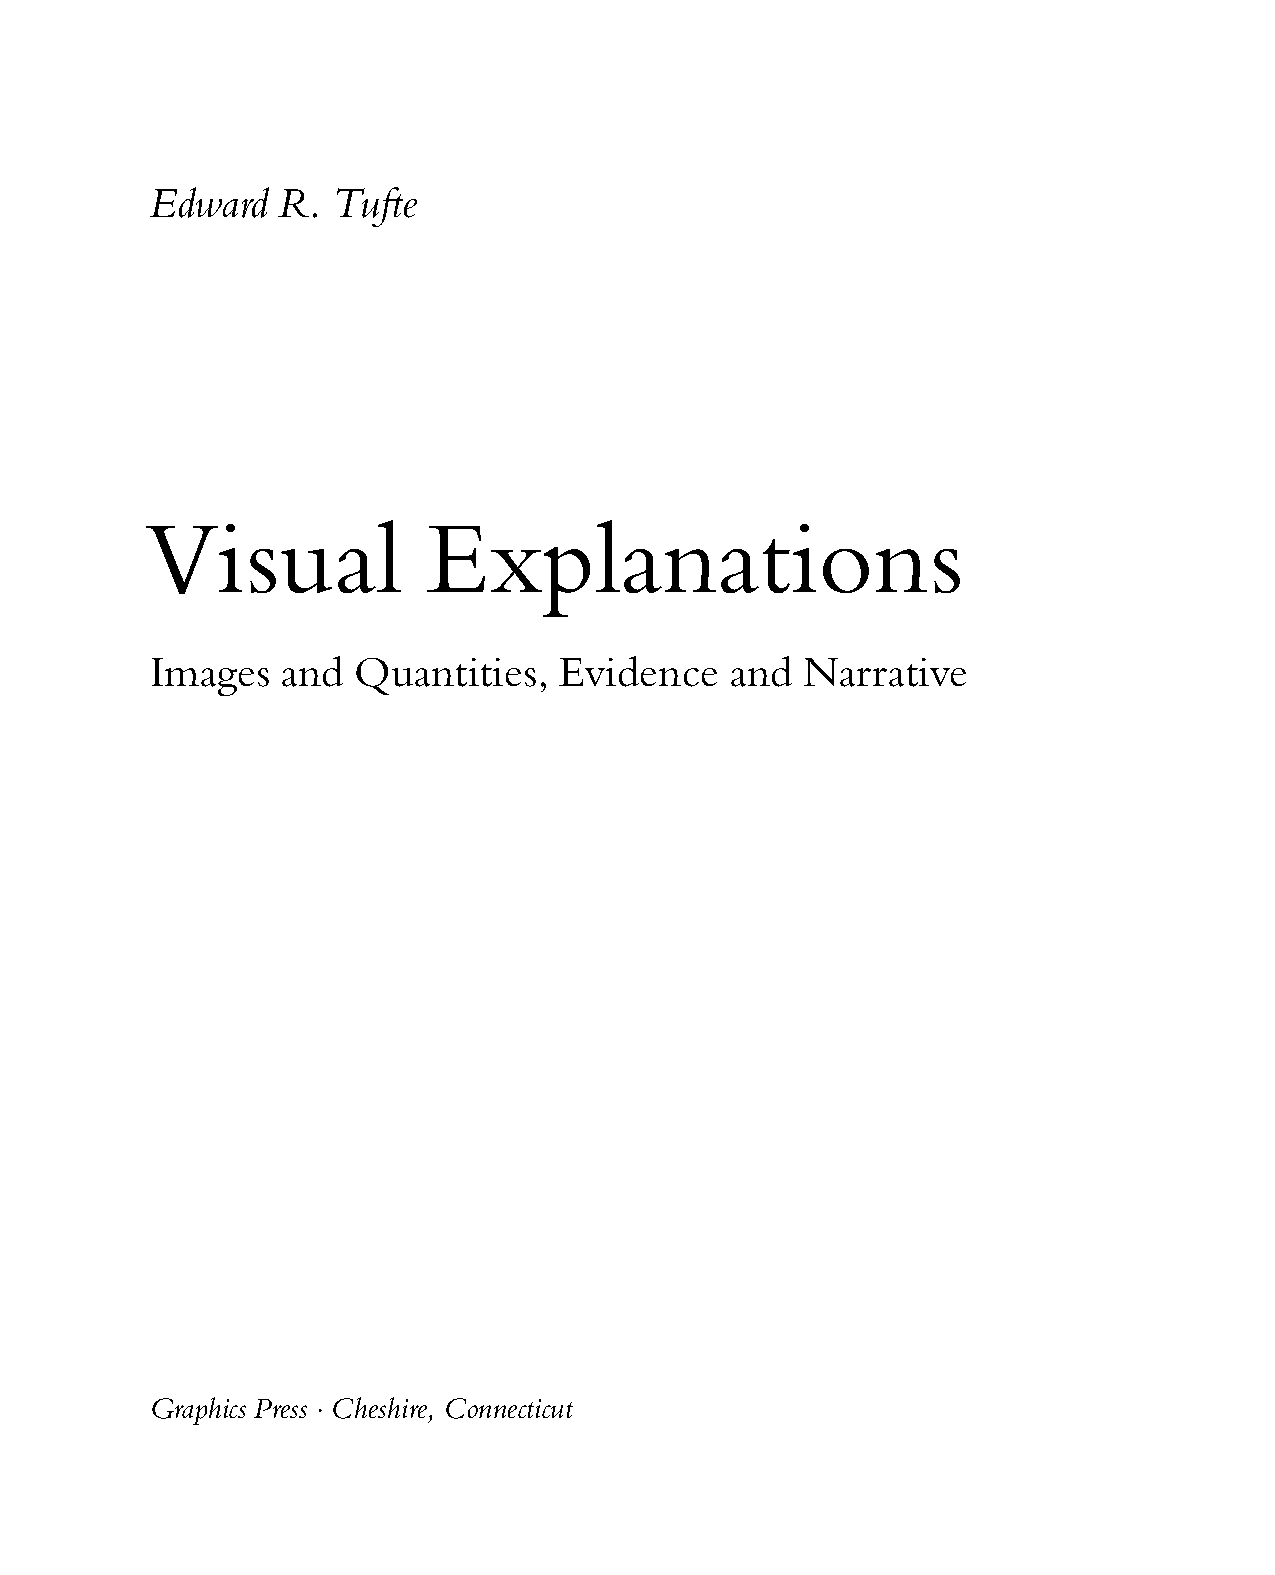
\includegraphics[width=0.45\linewidth]{graphics/ve-title.pdf}}
\hfill
\fbox{
\includegraphics[width=0.45\linewidth]{graphics/be-title.pdf}}
\end{figure*}

\newthought{The tables of contents} in Tufte's books give us our first
glimpse of the structure of the main matter.  \VDQI is split into two
parts, each containing some number of chapters.  His other three books only
contain chapters---they're not broken into parts.

\begin{figure*}[p]
\fbox{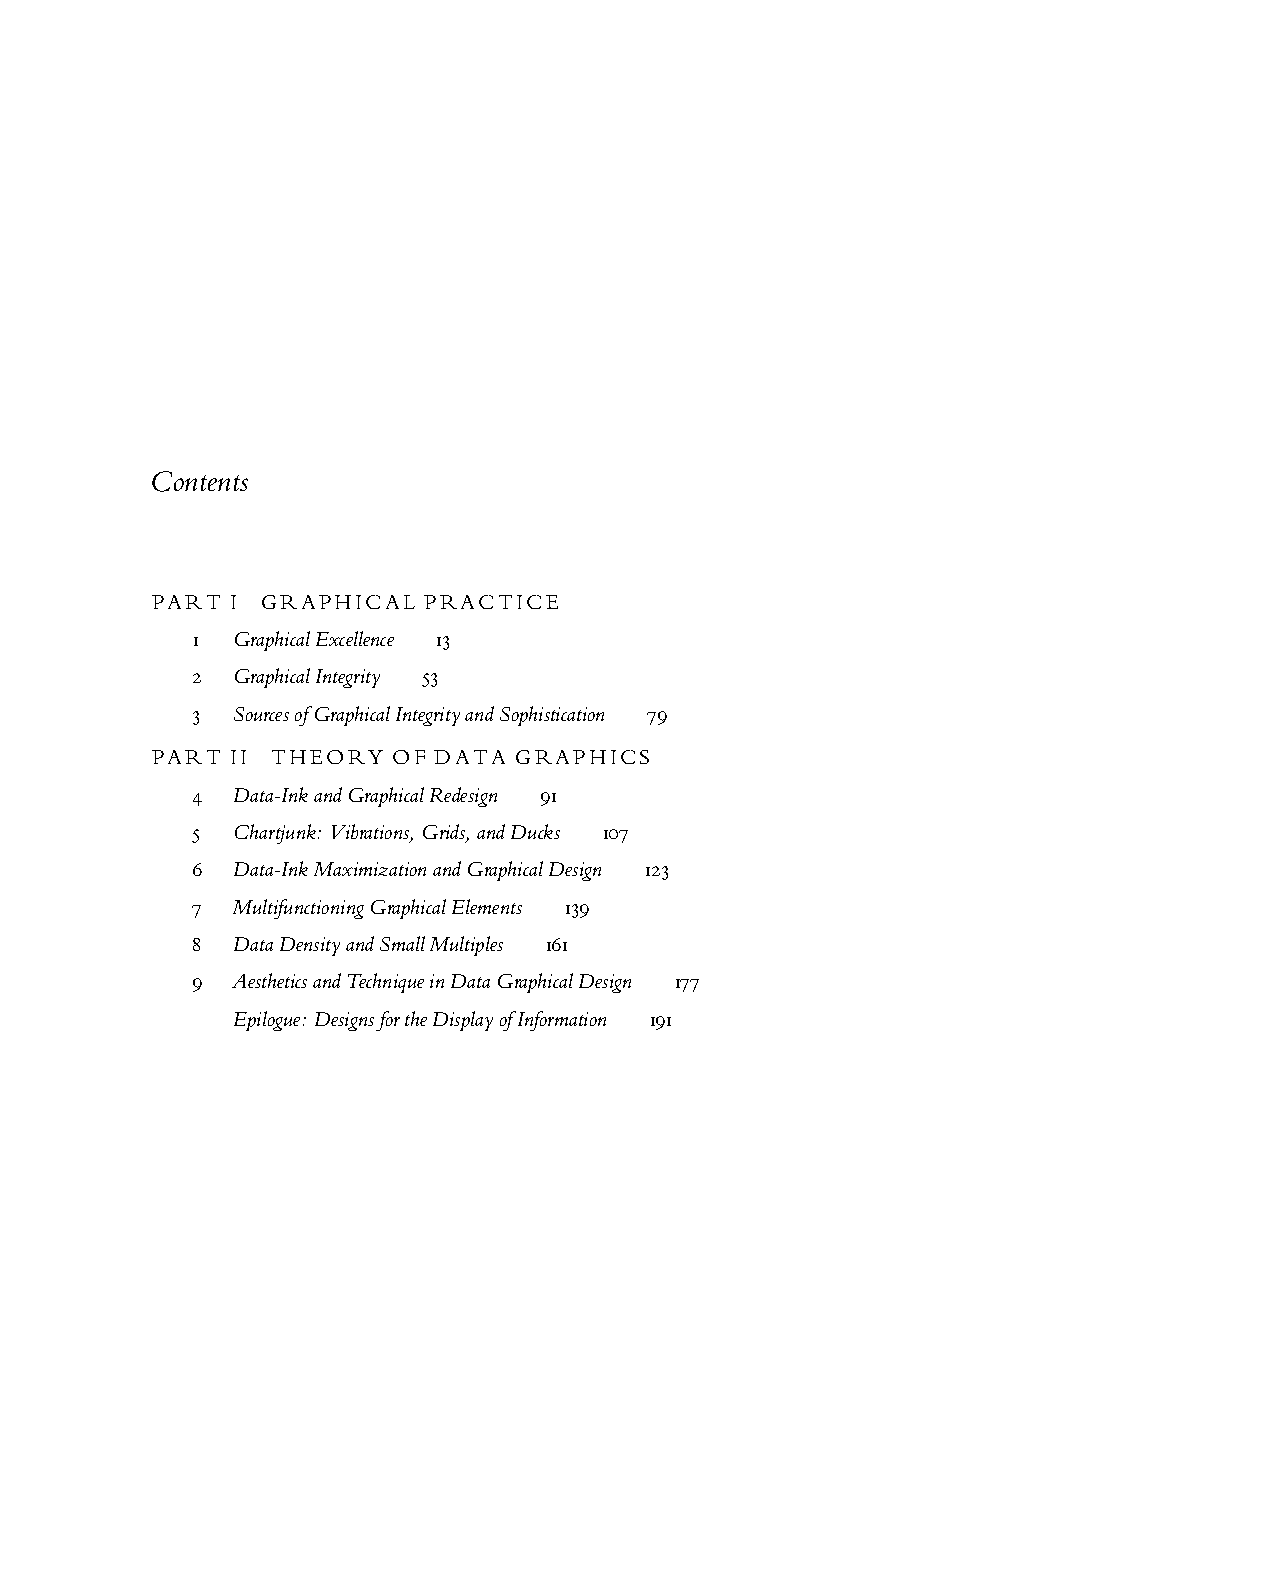
\includegraphics[width=0.45\linewidth]{graphics/vdqi-contents.pdf}}
\hfill
\fbox{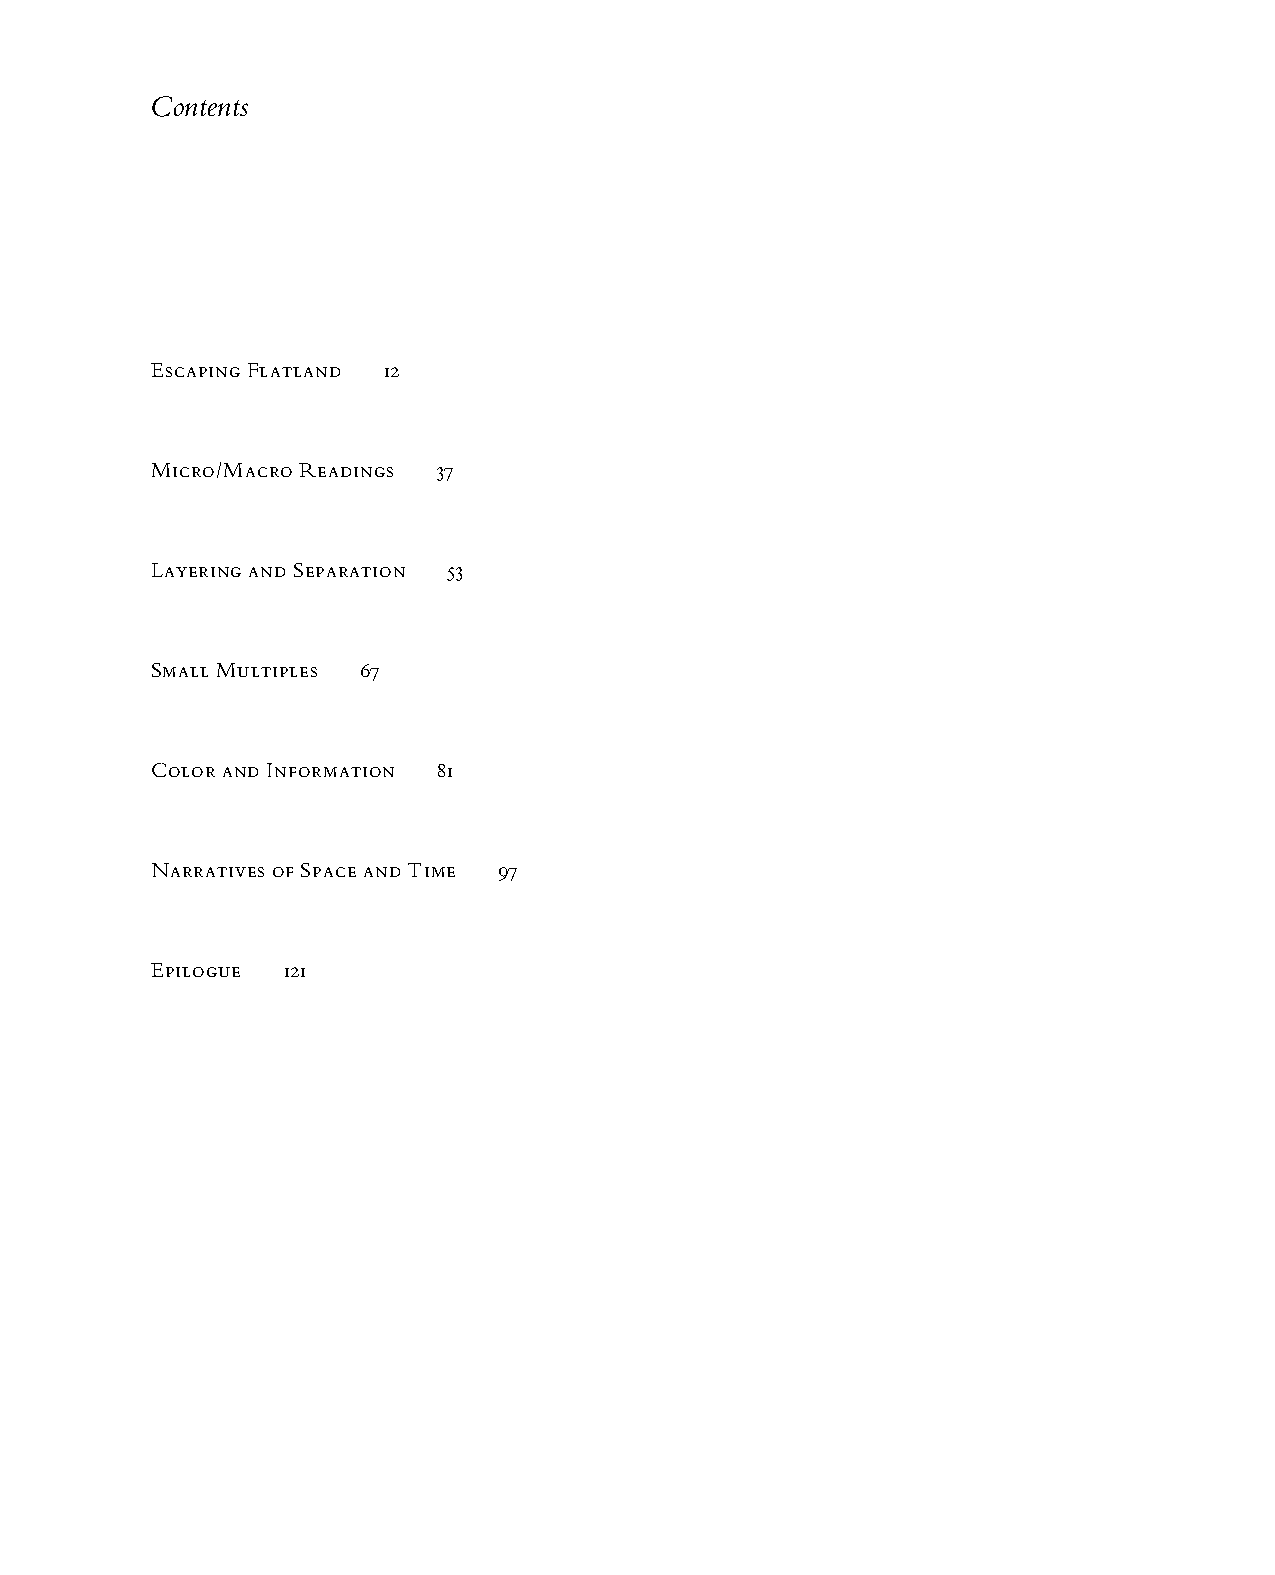
\includegraphics[width=0.45\linewidth]{graphics/ei-contents.pdf}}
\\\vspace{\baselineskip}
\fbox{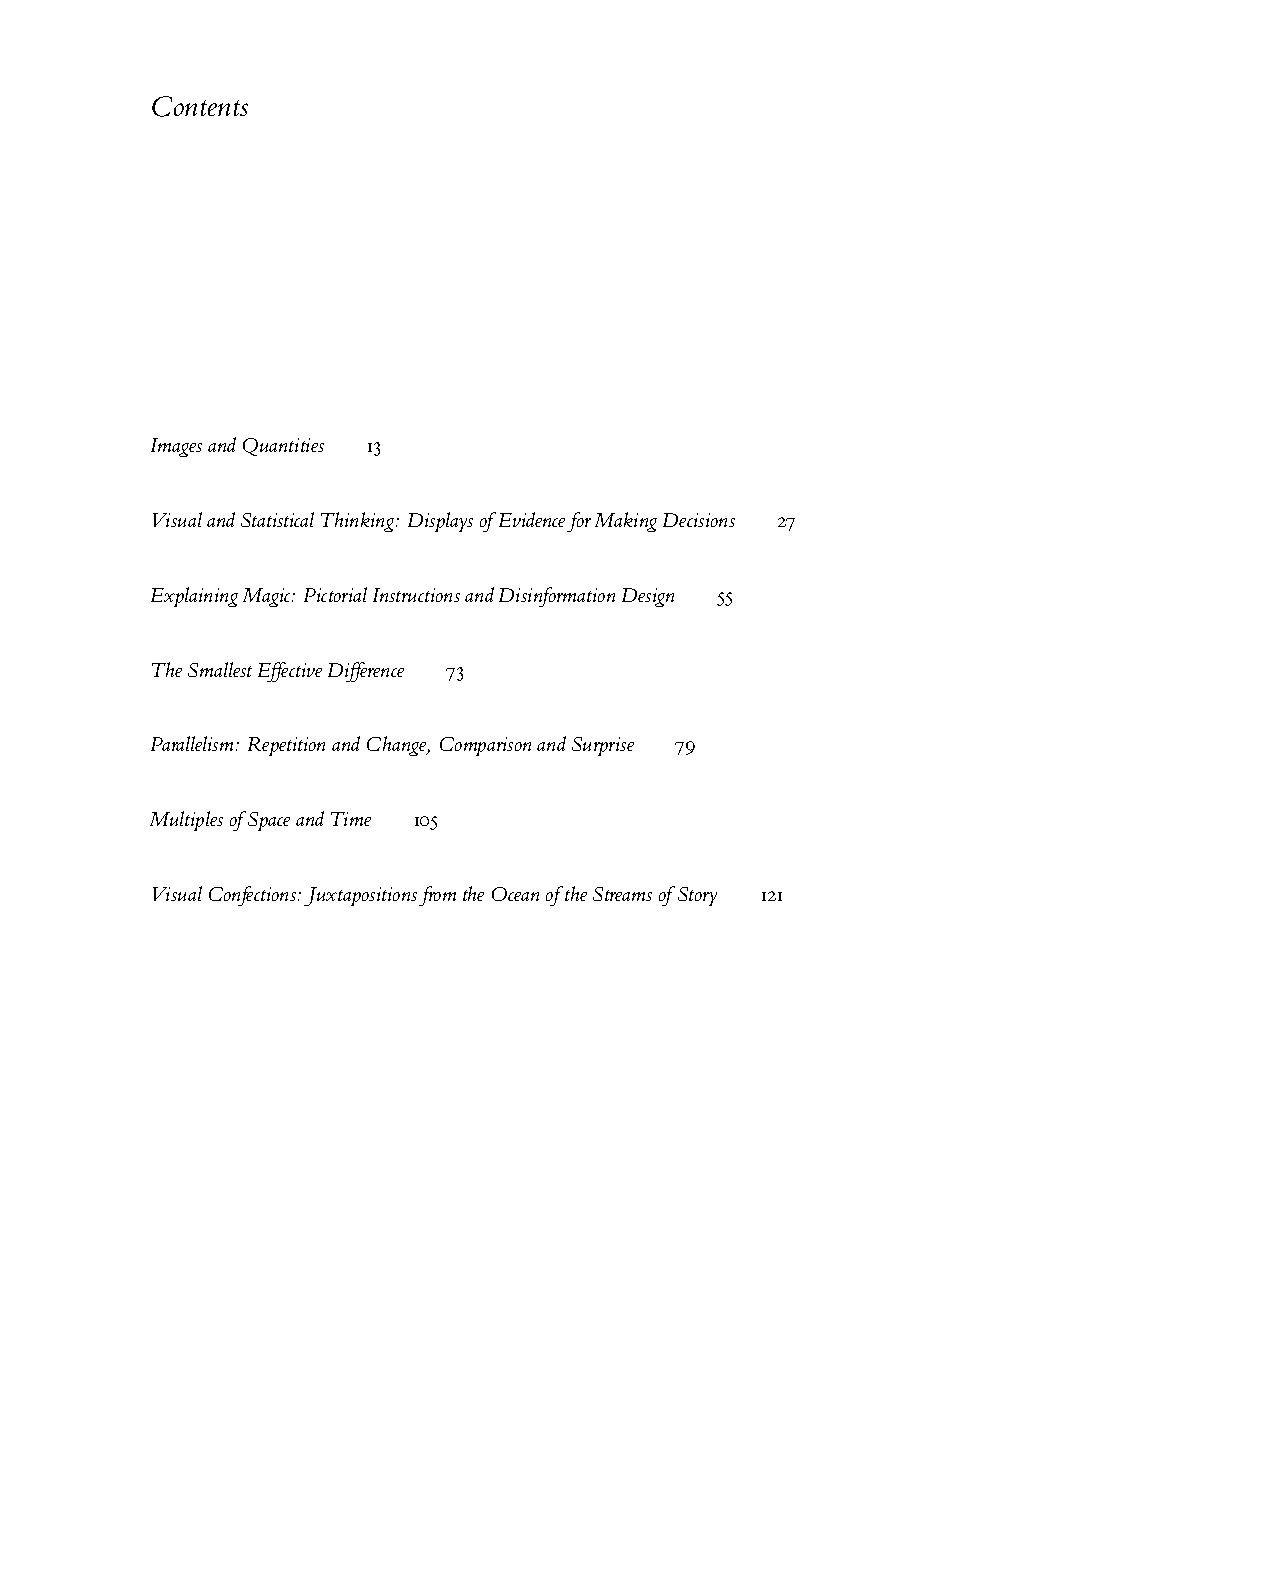
\includegraphics[width=0.45\linewidth]{graphics/ve-contents.pdf}}
\hfill
\fbox{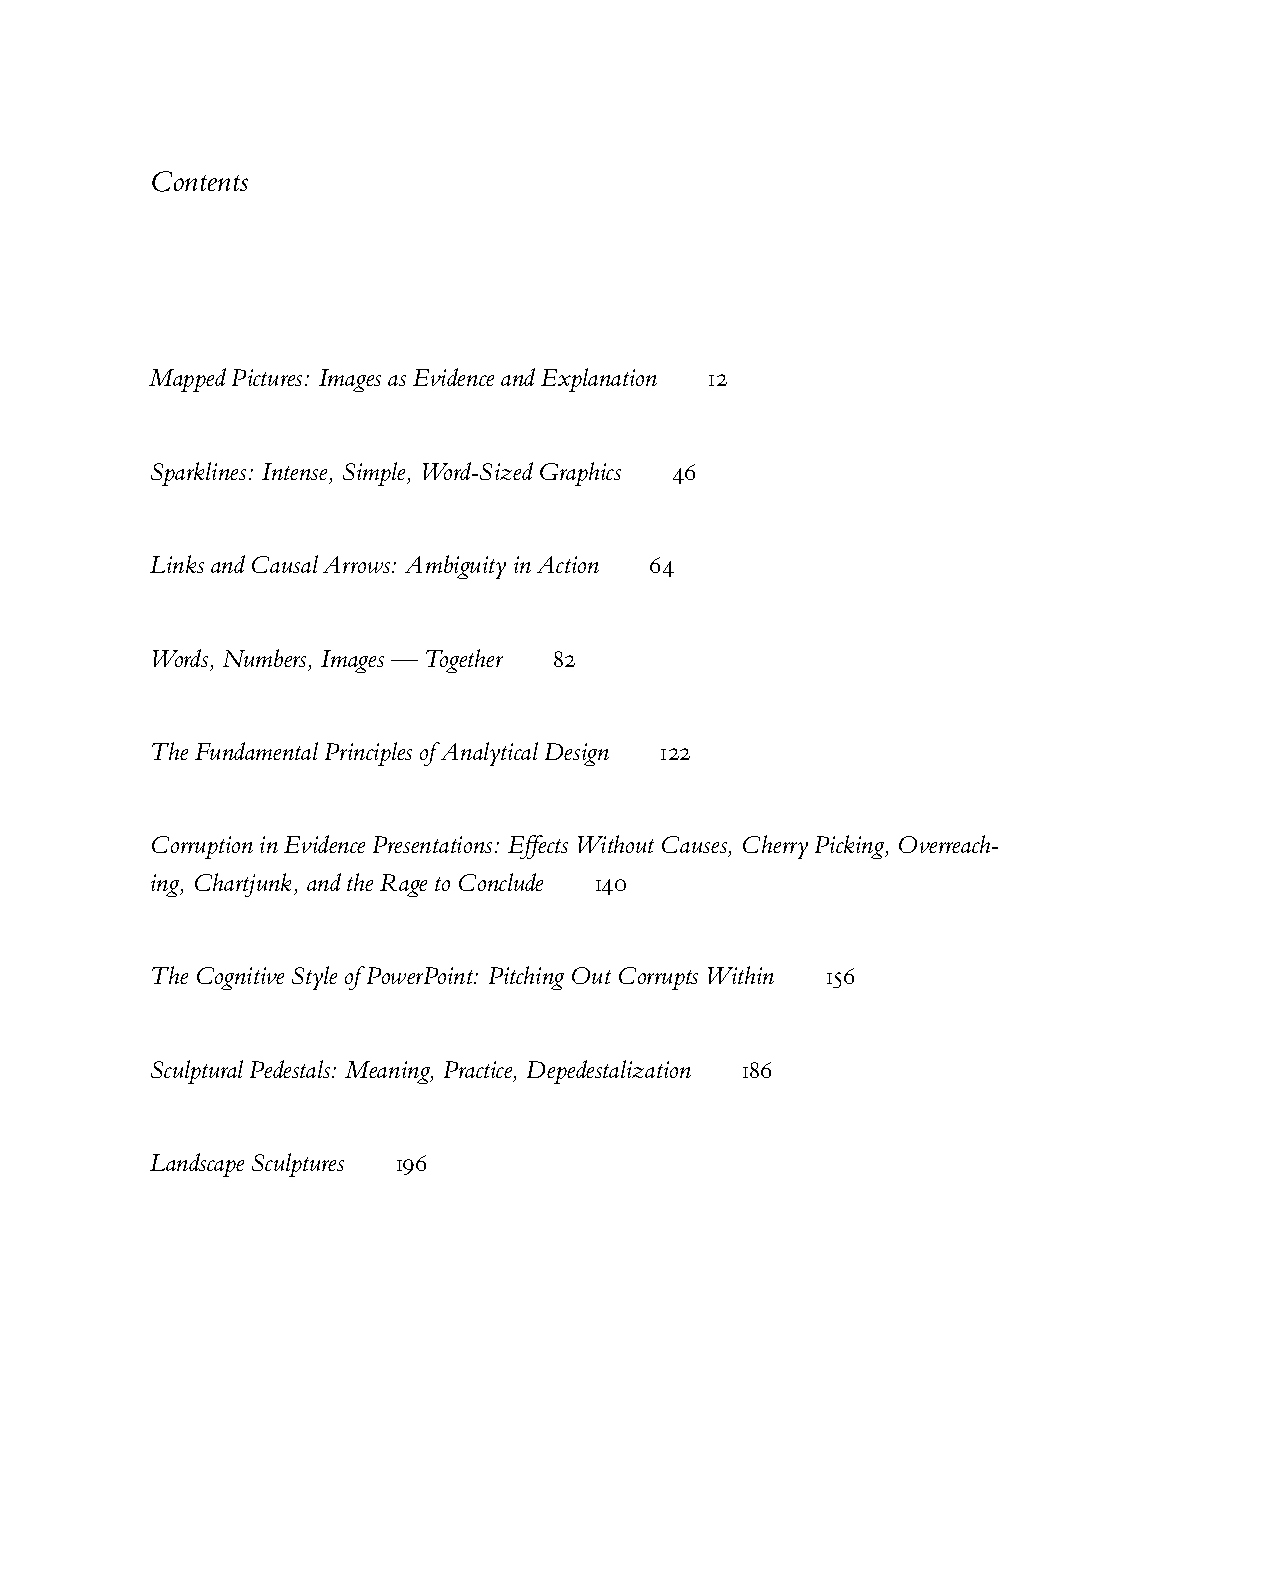
\includegraphics[width=0.45\linewidth]{graphics/be-contents.pdf}}
\end{figure*}


\section{Typefaces}

Tufte's books primarily use two typefaces: Bembo and Gill Sans.  Bembo is used
for the headings and body text, while Gill Sans is used for the title page and
opening epigraphs in \BE.

Since neither Bembo nor Gill Sans are available in default \LaTeX{}
installations, the \TL document classes default to using Palatino and
Helvetica, respectively.  In addition, the Bera Mono typeface is used for
\texttt{monospaced} type.

The following font sizes are defined by the \TL classes:

\begin{table}[h]
  \footnotesize%
  \begin{center}
    \begin{tabular}{lccl}
      \toprule
      \LaTeX{} size & Font size & Leading & Used for \\
      \midrule
      \verb+\tiny+         &  5 &  6 & sidenote numbers \\
      \verb+\scriptsize+   &  7 &  8 & --- \\
      \verb+\footnotesize+ &  8 & 10 & sidenotes, captions \\
      \verb+\small+        &  9 & 12 & quote, quotation, and verse environments \\
      \verb+\normalsize+   & 10 & 14 & body text \\
      \verb+\large+        & 11 & 15 & \textsc{b}-heads \\
      \verb+\Large+        & 12 & 16 & \textsc{a}-heads, \textsc{toc} entries, author, date \\
      \verb+\LARGE+        & 14 & 18 & handout title \\
      \verb+\huge+         & 20 & 30 & chapter heads \\
      \verb+\Huge+         & 24 & 36 & part titles \\
      \bottomrule
    \end{tabular}
  \end{center}
  \caption{A list of \LaTeX{} font sizes as defined by the \TL document classes.}
  \label{tab:font-sizes}
\end{table}

\section{Headings}

Tufte's books include the following heading levels: parts,
chapters,\sidenote{Parts and chapters are defined for the \texttt{tufte\-book}
class only.}  sections, subsections, and paragraphs.  Not defined by default
are: sub-subsections and subparagraphs.

\begin{table}[h]
  \begin{center}
    \footnotesize%
    \begin{tabular}{lcr}
      \toprule
      Heading & Style & Size \\
      \midrule
      Part & roman & \measure{24}{36}{40} \\
      Chapter & italic & \measure{20}{30}{40} \\
      Section & italic & \measure{12}{16}{26} \\
      Subsection & italic & \measure{11}{15}{26} \\
      Paragraph & italic & 10/14 \\
      \bottomrule
    \end{tabular}
  \end{center}
  \caption{Heading styles used in \BE.}
  \label{tab:heading-styles}
\end{table}

\section{Environments}

The following characteristics define the various environments:


\begin{table}[h]
  \begin{center}
    \footnotesize%
    \begin{tabular}{lcl}
      \toprule
      Environment & Font size & Notes \\
      \midrule
      Body text & \measure{10}{14}{26} & \\
      Block quote & \measure{9}{12}{24} & Block indent (left and right) by \unit[1]{pc} \\
      Sidenotes & \measure{8}{10}{12} & Sidenote number is set inline, followed by word space \\
      Captions & \measure{8}{10}{12} &  \\
      \bottomrule
    \end{tabular}
  \end{center}
  \caption{Environment styles used in \BE.}
  \label{tab:environment-styles}
\end{table}


\chapter{On the Use of the \texttt{tufte-book} Document Class}
\label{ch:tufte-book}

The \texttt{tufte-book} document class is modeled primarily on \BE, since
it's the most recent of Tufte's books and the design is (presumably) more
refined.

%This choice of book design has a few important implications:
%\begin{inparaenum}
%\item there are no parts---the highest heading level is the chapter;
%\item the use of a sans serif font for many design elements (especially the
%title page and epigraphs); and
%\item \emph{something else---yyy}.
%\end{inparaenum}



%%
% The back matter contains appendices, indices, glossaries, etc.

\backmatter



\bibliography{sample-handout}
\bibliographystyle{plainnat}

\end{document}

